\title{Discussion 1}
\author{0616014 楊政道}
\maketitle
\thispagestyle{fancy}
\section{辨認下列圖中電阻的電阻值}
\subsection{電阻A}
\begin{center} 
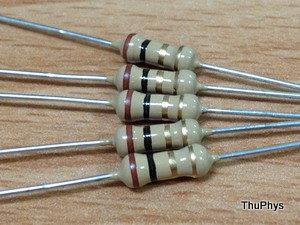
\includegraphics[width=5cm]{A.jpg} 
\end{center} 
\subsubsection{列出圖中電阻的顏色}
\paragraph{}
棕色, 黑色, 金色, 金色
\subsubsection{計算出電阻的電阻值}
\paragraph{}
$(10 \times 0.1\Omega) \pm 5\% = 1\Omega \pm 5\%$

\subsection{電阻B}
\begin{center} 
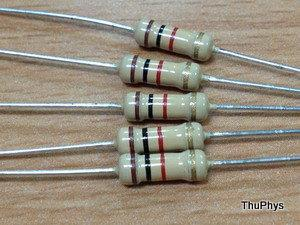
\includegraphics[width=5cm]{B.jpg} 
\end{center} 
\subsubsection{列出圖中電阻的顏色}
\paragraph{}
棕色, 黑色, 紅色, 金色
\subsubsection{計算出電阻的電阻值}
\paragraph{}
$(10 \times 100\Omega) \pm 5\% = 1000\Omega \pm 5\%$

\subsection{電阻C}
\begin{center} 
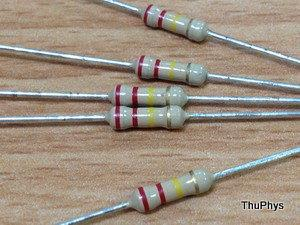
\includegraphics[width=5cm]{C.jpg} 
\end{center} 
\subsubsection{列出圖中電阻的顏色}
\paragraph{}
紅色, 紅色, 黃色, 金色
\subsubsection{計算出電阻的電阻值}
\paragraph{}
$(22 \times 10000\Omega) \pm 5\% = 220000\Omega \pm 5\%$
